\cotefile{156-8}
\scanpage{114}
\mspage{105}
% archive sheet number: 114 (upper left)
% L1
Je vais prouver
\[
\begin{aligned}
Z<X&\Longrightarrow Z\in\operatorname{supp}^{\circ}(\Phi)\\
Z>X&\Longrightarrow Z\in\operatorname{supp}^{\circ}(\Psi).
\end{aligned}
\]
% L4-6
\deleted{Pour ceci,} Prouvons p. ex. le premier, $Z<\unsure{x|X}$ (et \inserted{\unsure{ou simplement}} $Z\in\operatorname{supp}^{\circ}(\Phi\cup\Psi)$)
Soit donc
\[
Z'\in\operatorname{cosupp}^{\circ}(\Phi),\quad\text{i.e.}\quad Z'\mathrel{\mid\circ\mid}\Phi
\]
% L7-10
nous \deleted{\unsure{allons}} devons prouver $Z\mathrel{\unsure{\rangle\circ\mid|\mid\circ\mid}}Z'$. Nous \deleted{Soit} savons que c'est gagné si $Z'\mathrel{\mid\circ\mid}\Phi\cup\Psi$ \inserted{\unsure{resp.} $Z\mathrel{\mid\circ\mid}\Psi$ \unsure{aussi}} (et non seulement $Z'\mathrel{\mid\circ\mid}\Phi$).

% L11-15
\deleted{Mais soit}

\unsure{Quitte à|Cas A} : ``\unsure{agrandir}'' $X$, \unsure{on}
\[
\delta X=\{\underbrace{\operatorname{ex}\delta\Phi}_{a},\underbrace{\operatorname{or}\delta\Psi}_{b}\}
\]
i.e.
\[
\left\{\begin{aligned}
\deleted{\unsure{S}}X&=P_a&&\text{si}\quad a=b\\
X&=S_{ab}&&\text{si}\quad a<b
\end{aligned}\right.
\]
% L16-27
\deleted{\illegible{1}} Comme $Z'\mathrel{\mid\circ\mid}\Phi$, il s'ensuit aisément que $Z'\mathrel{\mid\circ\mid}P_a$ \uline{ou} $Z'=P_a$ \unsure{.}

% slanted
\margin{\uline{Lemme} \inserted{(\unsure{trivial})} $Z'\mathrel{\mid\circ\mid}Y$, et $\deleted{\unsure{P}}P\mathrel{\unsure{\triangleleft|\unlhd}}Y$ alors $Z'\mathrel{\unsure{\parallel|\mid\circ\mid}}P$ \uline{ou} $Z'=\deleted{\unsure{\{}}P\deleted{\unsure{\}}}$}

(Car on aura $\delta\Phi\cup\delta Z'\in\operatorname{Drap}(\unsure{\mathcal{L}|L})$, a fortiori $\delta\deleted{\unsure{\Phi}}Z'\cup\{P_a\}\in\operatorname{Drap}\mathcal{L}$, \deleted{\unsure{si on}} Si on avait $Z'=\deleted{\unsure{\{}}P_a$, \unsure{aurions|avions} par hypothèse $P_a\unsure{\ne|=|\in}Z'\mathrel{\mid\circ\mid}\Phi$, et $P_a\mathrel{\mid\circ\mid}\Psi$ puisque $X<\Psi$, on a $Z'\mathrel{\mid\circ\mid}\Phi\cup\Psi$, et on gagne. Sinon On aura $Z'<_{\mathrm{pos}}P_a$ ou $Z'>_{\mathrm{pos}}P_a$. Si $Z'<_{\mathrm{pos}}P_a$, on aura $Z'<_{\mathrm{pos}}\Psi$, donc $Z'\parallel\Psi$, on gagne encore.

% slanted
\margin{\uline{Lemme} (trivial) $X<_{\mathrm{pos}}\Psi\Longrightarrow\unsure{\operatorname{or.}X|\operatorname{or}_i X}<_{\mathrm{pos}}\Psi$}
\scanpage{115}
\mspage{106}
% archive sheet number: 115 (lower left)
% L1-4
Reste le cas $\deleted{\unsure{Z'>}}P_a\inserted{<Z'}$. Mais comme $Z<X$, on aura $Z\leq P_a$ ou \deleted{\unsure{$Z\leq P_a$|$Z<P_a$}}, donc on aura $Z<Z'$, d'où encore $Z\mathrel{\mid\circ\mid}Z'$, qed

% L5-8
\uline{NB} Je n'ai pas eu à utiliser Hyp., \deleted{ni la \unsure{constructibilité} de $\Phi$} mais \deleted{la} j'ai utilisé \deleted{\unsure{la const.|le contre}} que $\Phi$ $\Psi$ sont des \unsure{préfigures}.

% L9-14
\uline{Dém de (b)} Résulte par récurrence \inserted{(sur $\operatorname{card}\delta\Phi$)} de $1^{\circ}$, et du \deleted{\unsure{Deux}}

\uline{Lemme} : \unsure{Soient|Soit} $a<b<c$, et $\Phi=\{S_{ab},P_b,S_{bc}\}$. Alors
\[
\operatorname{supp}^{\circ}(\Phi)=\operatorname{supp}^{\circ}(S_{ac})
\]
(Lemme de composition des segments).

% L15-20
\uline{Démonstration} Il suffit de voir que $\Phi$ et $S_{ac}$ ont \unsure{même|mêmes} $\operatorname{cosupp}^{\circ}$. \deleted{Soit} Cela résulte du résultat légèrement plus \deleted{\unsure{donc} $X$} précis :

% L21-23
Si $X\in\unsure{M|\mathcal{M}}$, on a
\[
\begin{aligned}
X<_{\mathrm{pos}}\Phi\quad\inserted{\text{(i.e. }X<S_{ab}\text{)}}&\Longleftrightarrow X<S_{ac}\\
X>_{\mathrm{pos}}\Phi\quad\inserted{\text{(i.e. }X>S_{bc}\text{)}}&\Longleftrightarrow X>S_{ac}
\end{aligned}
\]
\margin{trivial (\unsure{sans Hyp.})}
\scanpage{116}
\mspage{107}
% archive sheet number: 116 (lower left)
% L1-2
Ainsi, le théorème est établi. On en conclut que \deleted{\unsure{tout}}

% L3-13: the following block has long diagonal cancellation strokes.
\deleted{\uline{Corollaire} (\unsure{détermination|determination} des supports constructibles de $\unsure{M|\mathcal{M}}$). \deleted{Soit $X$}}

\deleted{1) Tout support constructible peut s'obtenir de la façon suivante : on prend une figure \deleted{\unsure{$f$}} $F=F_D$, $D=(T_1<_{\mathrm{pos}}T_2<\cdots<_{\mathrm{pos}}T_n)\in\operatorname{Drap}^{*}(\operatorname{Drap}^{*}(\unsure{\mathcal{L}|L}))$, et pour tout $T_i$, on prend une partie $\beta_i\subset\unsure{\partial|\delta}F_{T_i}=\partial T_i$. \deleted{\unsure{On lui}} On lui associe la partie constructible}
\[
\deleted{\Phi=\deleted{\unsure{F}}(F_D\setminus F_D\cap M_0)\cup\bigcup\beta_i=\bigcup_i((F_{T_i}\setminus F_{T_i}\cap M_0)\cup\beta_i)}
\]
\deleted{et}
\[
\deleted{\operatorname{supp}^{\circ}\Phi=\operatorname{Omb}^{\circ}(\Phi)}
\]
% L14-20: below the cancellation strokes.
Alors
\[
\operatorname{supp}^{\circ}\Phi=\operatorname{supp}^{\circ}\Phi'
\]
$\Phi'$ \unsure{déduit} de $\Phi$ en ``\unsure{recollant}'' les morceaux'', et ayant la propriété d'être \uline{``\unsure{non morcelée|non morcelé}''}
i.e.
\[
\forall x\in\Phi'\cap M_0,\quad\operatorname{card}\{X\in\Phi'\mid x\mathrel{\triangleleft}X\}\ne2
\]
(\uline{NB} Ce cardinal est \unsure{tjrs} $\in\{0,1,2\}$)

Ceci posé, on trouve.
\scanpage{117}
\mspage{108}
% archive sheet number: 117 (lower left)
% L1-3
\uline{Théorème} 1) Tout support constructible $S$ s'écrit sous la forme $\operatorname{supp}^{\circ}\Phi$, où $\Phi$ est une préfigure non morcelée\textsuperscript{*};
% slanted
\margin{* Je dis plutôt : ``\unsure{irredondante|irrédondante}''}
% L4-6
\deleted{\unsure{2)} Cette écriture est unique, et on a}
et pour une telle $\Phi$, on a
\[
\operatorname{supp}^{\circ}(\Phi)=\operatorname{Omb}^{\circ}(\unsure{\Psi|\Phi})=\bigcup_{X\in\Phi}\operatorname{Omb}^{\circ}(\deleted{\unsure{\Phi}}X)
\]
(\uuline{réunion} \uuline{disjointe}).
% L7-11
Les éléments de $\inserted{\Phi_1=}\Phi\cap\unsure{M|\mathcal{M}}_1$ sont les éléments de $S$ qui sont \deleted{maximaux} $1^{\circ})$ de dim 1 et $2^{\circ})$ maximaux dans $S$ pour $\overset{\circ}{\ll}$. \inserted{(ou pour $\ll$, c'est pareil)} Les éléments de $\Phi_0=\Phi\cap M_0$ sont \deleted{les éléments de $S\cap M_0$ qui sont \unsure{suivants} : \unsure{où|ou} bien ils sont} \inserted{caractérisés par}
\[
\Phi_0=\left(\bigcup_{X\in\Phi_1}\unsure{\partial|\delta}X\right)\cap\deleted{\unsure{\Phi}}S\cup\Phi_{0\,\mathrm{is}}\quad\deleted{\unsure{\phi}}
\]
% L12-16
(réunion disjointe), où \deleted{$\Phi_{0\,\mathrm{is}}$ est}
\[
\begin{aligned}
\Phi_{0\,\mathrm{is}}&=\text{ens des sommets isolés de }\Phi\\
&=\text{ens. des éléments de }S\cap M_0\text{ qui}\\
&\qquad\text{sont maximaux dans }S\text{ pour }\ll
\end{aligned}
\]
\deleted{\unsure{Ce qui}}

% L17-22
\deleted{\unsure{Ainsi}} En particulier, $\Phi$ est bien \unsure{déterminé|déterminée} par la connaissance de $S$. On dit que $S$ est \uline{fermé} si $\Phi$ est fermée, i.e. est une figure --- \unsure{ou.|ou} si $S$ est le support d'une figure.
\scanpage{118}
\mspage{109}
% archive sheet number: 118 (lower left)
% L1-4
2) Pour tout support constructible $S\inserted{\deleted{\unsure{S}}\Phi}$ il existe un plus petit support constructible fermé le contenant, \inserted{si $S=\operatorname{supp}^{\circ}\Phi$,} il est donné par
\[
S=\operatorname{supp}^{\circ}(\overline{\Phi})=\operatorname{supp}(\overline{\Phi})
\]
% slanted
\margin{À vérifier ! Facile : c'est aussi $\operatorname{supp}^{\circ}(\widetilde{S})$ \unsure{\{} et $=\unsure{\operatorname{sat.}|\operatorname{sat}}\widetilde{S}$ adhérence au sens de la \unsure{rel.} $\unlhd$ de $\unsure{M|\mathcal{M}}$\unsure{.}}
% L5-7
--- mais \unsure{ici on fera|on fera} attention que \deleted{\unsure{$=$ si $\Phi$}} $\overline{\Phi}$ peut fort bien être morcelée, même si $\Phi$ ne \deleted{\unsure{$S$}} l'est pas.

% left margin drawing, slanted in the manuscript
\figure{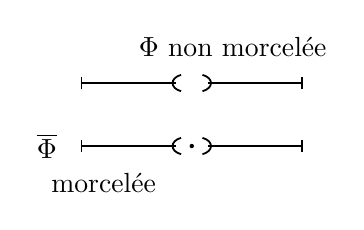
\begin{tikzpicture}[line width=.65pt,scale=.8]
\node at (2.4,.58) {$\Phi$ non morcelée};
\draw (0,0)--(1.5,0); \draw (2,0)--(3.5,0);
\draw (0,-.1)--(0,.1); \draw (3.5,-.1)--(3.5,.1);
\draw (1.58,.13) .. controls (1.40,.08) and (1.40,-.08) .. (1.58,-.13);
\draw (1.92,.13) .. controls (2.10,.08) and (2.10,-.08) .. (1.92,-.13);
\node at (-.55,-1) {$\overline{\Phi}$};
\draw (0,-1)--(1.5,-1); \draw (2,-1)--(3.5,-1);
\draw (0,-1.1)--(0,-.9); \draw (3.5,-1.1)--(3.5,-.9);
\draw (1.58,-.87) .. controls (1.40,-.92) and (1.40,-1.08) .. (1.58,-1.13);
\draw (1.92,-.87) .. controls (2.10,-.92) and (2.10,-1.08) .. (1.92,-1.13);
\fill (1.75,-1) circle (.035);
\node at (.35,-1.58) {morcelée};
\end{tikzpicture}}
% L8-10
3) Description combinatoire des supports constructibles via les préfigures non morcelées\textsuperscript{*}

% L11-17
\uline{4. juillet} Je voudrais donner une \unsure{paramétrisation} tant soit peu ``autoduale'' des supports constructibles, i.e. des préfigures non morcelées (ou ``\unsure{irredondantes|irrédondantes}''). Pour cela il faut ``mettre à part'' ses points isolés\inserted{de $\Phi$}, et les traiter en vis-à-vis des points de $\unsure{\mathcal{L}|L}$ qui \deleted{sont} ne sont pas dans $\Phi$, mais adhérents à $\Phi$ dans $M$\textsuperscript{\(\unsure{\lambda}\)}.
% slanted
\margin{$\unsure{\lambda}$ et \deleted{\unsure{pas}} $\notin\unsure{\partial|\delta}\Phi$ --- i.e. les ``points-frontière internes''}

On trouve ceci.

% L18-24
On regarde la figure \deleted{$\Phi_1=$} \deleted{$\overline{\Phi}\setminus\text{ens des points isolés}$} \deleted{de $\overline{\Phi}$}
\[
\Phi_1=\overline{\Phi}\setminus\{\text{ens des points isolés de }\overline{\Phi}\}
\]
c'est une figure qui \deleted{\unsure{n'est p}} peut ou pas être \unsure{irredondante|irrédondante}. Celle l'est sss \deleted{$\Phi$} \deleted{\unsure{ou|si} \unsure{que des|des} $\deleted{\unsure{\Phi}}\overline{\Phi}\setminus\Phi$ est formé de points de}
\[
\overline{\Phi}\setminus\Phi\subset\partial\Phi=\{s\in\delta\Phi\mid\text{ordre de }s\text{ dans }\overline{\Phi}\text{ est }1\}
\]
i.e. sss $\Phi$ n'a \deleted{\unsure{$\Phi$}} pas de point frontière interne
\scanpage{119}
\mspage{110}
% archive sheet number: 119 (lower left)
% Heading
\uline{Parenthèse} Zoologie des \uline{sommets} d'une préfigure.

% upper-left drawing
\figure{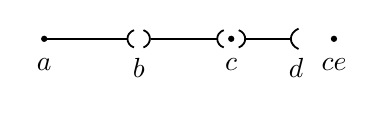
\begin{tikzpicture}[line width=.65pt]
\draw (0,0)--(1.05,0); \draw (1.35,0)--(2.2,0); \draw (2.55,0)--(3.15,0);
\fill (0,0) circle (.04); \fill (2.375,0) circle (.04); \fill (3.68,0) circle (.04);
\draw (1.14,.11) .. controls (1.03,.07) and (1.03,-.07) .. (1.14,-.11);
\draw (1.26,.11) .. controls (1.37,.07) and (1.37,-.07) .. (1.26,-.11);
\draw (2.28,.11) .. controls (2.17,.07) and (2.17,-.07) .. (2.28,-.11);
\draw (2.47,.11) .. controls (2.58,.07) and (2.58,-.07) .. (2.47,-.11);
\draw (3.23,.13) .. controls (3.10,.07) and (3.10,-.07) .. (3.23,-.13);
\node[below] at (0,-.12) {$a$}; \node[below] at (1.2,-.12) {$b$};
\node[below] at (2.375,-.12) {$c$}; \node[below] at (3.2,-.12) {$d$};
\node[below] at (3.68,-.12) {$\deleted{\unsure{c}}e$};
\end{tikzpicture}}
\[
\begin{aligned}
\Phi&=\{\deleted{\unsure{P}}_a,S_{ab},S_{bc},\deleted{\unsure{P}}_{\unsure{d|c}}\deleted{\unsure{\{}}S_{cd},e\}\\
\overline{\Phi}&=\{\deleted{\unsure{P}}_a,S_{ab},\deleted{\unsure{P}}_b,S_{bc},\deleted{\unsure{P}}_c,\deleted{\unsure{P}}S_{c\deleted{\unsure{b}}d},d,e\}\\
\partial\Phi&=\{a,d\}
\end{aligned}
\]
% Upper-right block: cancelled with several diagonal strokes.
\deleted{$\delta\Phi$ (ens. des sommets de $\Phi$) $=\overline{\Phi}\cap\unsure{\mathcal{L}|L}=(\overline{\Phi})_0$}

\deleted{sommets \uline{propres} : $\delta\Phi\cap\Phi_0$, \uline{impropres} $\delta\Phi\cap\mathcal{L}$}
\[
\deleted{\operatorname{ord}(\underset{\substack{\uparrow\\\mathcal{L}}}{a},\Phi)=\operatorname{card}(\{X\in\unsure{M|\mathcal{M}}\cap\Phi=\Phi_1\mid a\triangleleft X)}
\]
\[
\deleted{\delta\Phi=\{a\in\mathcal{L}\mid\operatorname{ord}(a,\Phi)=}
\]
\deleted{sommet isolé de $\Phi$ : d'ordre 0}

\deleted{sommet bord de $\Phi$ : d'ordre 1}
\[
\deleted{\text{deux cas }\left\{\begin{aligned}a\in\Phi&\quad\text{sommet bord propre}\\a\notin\Phi&\quad\text{sommet bord impropre}\end{aligned}\right.}
\]

% L10-14, full-width text
Rappels
\[
\delta\Phi\ (\text{ensemble des \uline{sommets} de }\Phi)=\overline{\Phi}\cap\mathcal{L}=(\overline{\Phi})_0
\]
sommets \uline{propres} : ceux de $\Phi_0=\overline{\Phi}\cap\mathcal{L}\subset\delta\Phi$

sommets impropres : ceux qui ne sont pas dans $\Phi_0$
\[
\operatorname{ord}(\underset{\substack{\uparrow\\\mathcal{L}}}{a},\Phi)=\operatorname{card}(\{X\in\underset{\inserted{\substack{\Vert\\M\cap\mathcal{L}}}}{\Phi_1}\mid a\triangleleft X)\in\{0,1,2\}.
\]
% L15-17
(\uline{ordre de} $a$ \uline{p.r. à} $\Phi$) Cet ordre est zéro si $a$ n'est pas un sommet, mais il peut être zéro aussi pour un sommet de $\Phi$, \deleted{\unsure{car}}

% L18-20
\uline{Lemme} Si $a\in\delta\Phi$, \deleted{alors}\inserted{et} $\operatorname{ord}(a,\Phi)=0$, on a $a\in\Phi$.
Un tel sommet de $\Phi$ est dit \deleted{\unsure{isolé}}\uline{sommet isolé}.
\[
\Phi_{\mathrm{is}}=\{a\in\delta\Phi\mid\operatorname{ord}(a,\Phi)=0\}\subset\Phi_0
\]
% L21-25
Les sommets d'ordre 1 sont les \uline{sommets-bord}
\[
\partial\Phi=\{\underset{\inserted{\text{ou }s\in\mathcal{L}}}{s\in\delta\Phi}\mid\operatorname{ord}(\unsure{a|s},\Phi)=1\}
\]
Parmi ces sommets\inserted{-bord} on distingue les sommets-bord propres, et impropres
\[
\underbrace{\Phi_0\cap\partial\Phi=\partial_0\Phi}_{\substack{\text{sommets-bord}\\\text{propres}}}\subset\Phi
\]
\deleted{\unsure{$P$}}

Les sommets d'ordre 2 sont les \uline{sommets} \uline{internes}
\[
\deleted{\unsure{\delta}}\delta_{\mathrm{int}}(\Phi)=\{\underset{\inserted{\text{ou }s\in\mathcal{L}}}{s\in\delta\Phi}\mid\operatorname{ord}(s,\Phi)=2\}
\]
\scanpage{120}
\mspage{111}
% archive sheet number: 120 (lower left)
% L1-4
Parmi les sommets internes, on distingue les sommets propres, ou \uline{sommets} \uline{redondants} ou ``sommets de morcellement'', et les sommets impropres, ou \uline{sommets} \uline{lacunaires}.

Dans la préfigure
\figure{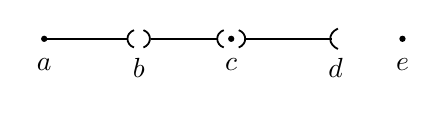
\begin{tikzpicture}[line width=.65pt]
\draw (0,0)--(1.05,0); \draw (1.35,0)--(2.2,0); \draw (2.55,0)--(3.65,0);
\fill (0,0) circle (.04); \fill (2.375,0) circle (.04); \fill (4.55,0) circle (.04);
\draw (1.14,.11) .. controls (1.03,.07) and (1.03,-.07) .. (1.14,-.11);
\draw (1.26,.11) .. controls (1.37,.07) and (1.37,-.07) .. (1.26,-.11);
\draw (2.28,.11) .. controls (2.17,.07) and (2.17,-.07) .. (2.28,-.11);
\draw (2.47,.11) .. controls (2.58,.07) and (2.58,-.07) .. (2.47,-.11);
\draw (3.73,.13) .. controls (3.60,.07) and (3.60,-.07) .. (3.73,-.13);
\node[below] at (0,-.12) {$a$}; \node[below] at (1.2,-.12) {$b$};
\node[below] at (2.375,-.12) {$c$}; \node[below] at (3.7,-.12) {$d$};
\node[below] at (4.55,-.12) {$e$};
\end{tikzpicture}}
il y a un sommet de chacun des cinq types combinatoires
\diagram{\(\begin{array}{ll}
\text{sommet isolé}&e\\
\text{sommet bord propre}&a\\
\text{\rule{2.4cm}{.3pt}\ impropre}&d\\
\text{sommet interne propre ou redondant}&c\\
\text{sommet interne impropre ou lacunaire}&b
\end{array}\)}

% L12-17
\deleted{\unsure{Pour que intervalles}}
Je préfère à présent appeler $S_{a,b}=S_{b,a}$ ou $S_{\{a,b\}}$ un intervalle (plutôt qu'un segment). Le \uline{segment} associé à l'intervalle est $\widetilde{S}_{a,b}=\{S_{ab},a,b\}$ --- c'est le \unsure{multistrate} complet associé à $S_{ab}$.

\deleted{\unsure{Si} $X\in\Phi_{\unsure{T_D|D}}$} On a posé
\[
\underbrace{\Phi_0\unsure{>|=}\Phi\cap\unsure{M|\mathcal{M}}_0=\Phi\cap\unsure{\mathcal{L}|L}}_{\substack{\text{ou ens. des sommets}\\\text{propres.}}},\quad\Phi_1=\Phi\cap M_1
\]
% L18-end: cancelled by long diagonal strokes.
\deleted{Pour les éléments de $\Phi_1$, ou \uline{intervalles de $\Phi$}, on distingue les intervalles de $\Phi$ tels que $\widetilde{X}\subset\Phi$ i.e. $\overline{X}\subset\Phi$ \inserted{i.e. $\unsure{\partial|\delta}X\subset\Phi_0$} (on peut les appeler \uline{fermés} \uline{dans} $\Phi$), \deleted{et} ceux pour lesquels $\partial X\cap\Phi_0=\{a\}$ (\uline{semi}-\uline{ouverts} \unsure{droits|droit}}
